\documentclass[12]{article}
\usepackage{listings}
\usepackage{color}
\usepackage{caption}
\definecolor{maroon}{rgb}{0.5,0,0}
\definecolor{darkgreen}{rgb}{0,0.5,0}
\definecolor{lightgray}{rgb}{0.95, 0.95, 0.95}
\definecolor{darkgray}{rgb}{0.4, 0.4, 0.4}
\definecolor{purple}{rgb}{0.65, 0.12, 0.82}
\usepackage{caption}

\lstdefinelanguage{CSS}{
    keywords={color,background-image,margin,padding,font,weight,display,position,top,left,right,bottom,list,style,border,size,white,space,min,width, transform, transition, transition-property, transition-duration, transition-timing-function},
    alsodigit={-},
    sensitive=true,
    morecomment=[l]{//},
    morecomment=[s]{/*}{*/},
    morestring=[b]',
    morestring=[b]"
}
\lstdefinelanguage{XML}
{
  basicstyle=\ttfamily,
  morestring=[s]{"}{"},
  morecomment=[s]{?}{?},
  morecomment=[s]{!--}{--},
  commentstyle=\color{darkgreen},
  moredelim=[s][\color{black}]{>}{<},
  moredelim=[s][\color{red}]{\ }{=},
  stringstyle=\color{blue},
  identifierstyle=\color{maroon}
}

\definecolor{javared}{rgb}{0.6,0,0} % for strings
\definecolor{javagreen}{rgb}{0.25,0.5,0.35} % comments
\definecolor{javapurple}{rgb}{0.5,0,0.35} % keywords
\definecolor{javadocblue}{rgb}{0.25,0.35,0.75} % javadoc
 
\lstset{language=Java,
basicstyle=\ttfamily,
keywordstyle=\color{javapurple}\bfseries,
stringstyle=\color{javared},
commentstyle=\color{javagreen},
morecomment=[s][\color{javadocblue}]{/**}{*/},
numbers=left,
numberstyle=\tiny\color{black},
numbersep=10pt,
tabsize=4,
showspaces=false,
showstringspaces=false}


\usepackage{subcaption}



\usepackage{Graphicx}

\usepackage{setspace}
\newcommand{\hsp}{\hspace{20pt}}
\newcommand{\HRule}{\rule{\linewidth}{0.5mm}}
\usepackage{minitoc}


\begin{document}
\onehalfspacing


\begin{titlepage}
  \begin{sffamily}
  \begin{center}

    
\includegraphics[scale=0.3]{C:/workplace/Java/project/inpt.png}~\\[1.5cm]

    \textsc{\LARGE Institut national des postes et télécommunications}\\[2cm]

    \textsc{\Large Rapport de projet}\\[1.5cm]

    % Title
    \HRule \\[0.4cm]
    { \huge \bfseries  Dynamic Web project :
    Psychologue en ligne \\[0.1cm] }

    \HRule \\[2cm]


    \begin{minipage}{0.4\textwidth}
      \begin{flushleft} \large
       Realisé par :\\
        Driouich Meryam\\
        Azzim Taha\\
      \end{flushleft}
    \end{minipage}
    \begin{minipage}{0.4\textwidth}
      \begin{flushright} \large
       Sous l'encadrement de :\\ \textbf{Dr Mahmoud Rlhamlaoui}
      \end{flushright}
    \end{minipage}

    \vfill

    % Bottom of the page
    {\large  Année universitaire :2020-2021}

  \end{center}
  \end{sffamily}
\end{titlepage}
\tableofcontents

\newpage




\section{Analyse et spécification des besoins}
\subsection{Introduction}
Pour assurer une bonne compréhension des différents fonctionnalités de notre projet, nous allons consacrer cette section pour identifier les acteurs de notre plateforme, cataloguer les besoins fonctionnels et les besoins non fonctionnels et terminer avec une présentation du diagramme des cas d'utilisation générale ainsi que le raffinement de chaque cas d'utilisation de notre application.

\subsection{Analyse des besoins}

 Notre but de cette partie est de définir avec détails l'ensemble des fonctionnalités offertes par l'application. Les besoins dégagés ont été répartis en deux catégories fonctionnnels et non fonctionnels.
 \subsubsection{Les besoins fonctionnels}
 
 Les besoins fonctionnels se sont les fonctionnalités du système. Ce sont d'autre part les besoins spécifiant un comportement d'entrée ou bien sortie du système, ces derniers sont classés par acteurs.
 
 \paragraph{Présentation des acteurs\\}
 
 Un acteur représente une personne ou un matériel ou un logiciel qui interagit d'une manière directer avec le système. Un acteur a le droit de consulter ou modifier directement l'état du système en émettant ou recevant des messages susceptible d'être porteur des données.\\
 
 Les acteurs qui interagient dans notre système sont:\\
 
 \begin{itemize}
 \item \textbf{Utilisateur:} Un utilisateur est déjà inscrit dans l'application,il peut répondre aux questions proposer par le psychologue et approuver par le RH.
 \item \textbf{Psychologue :} Ajoute un questionnaire et envoie des recommandations à l'utilisateur.
 \item \textbf{RH:} il approuve ou affecte le questionnaire à passer.
 \end{itemize}
 
 \paragraph{Les besoins fonctionnels par Acteur\\}
 
 Le tableau ci dessus représente les besoins fonctionnels de notre système:
 
 \begin{center}
 

 
\begin{tabular}{|l|l|}
\hline
Acteur      & Fonctionnalités                                                                                                                                                             \\ \hline
Utilisateur & \begin{tabular}[c]{@{}l@{}}-S'authentifier\\ -Répondre au questionnaire\end{tabular}                                                                                        \\ \hline
RH          & \begin{tabular}[c]{@{}l@{}}-S'authentifier\\ -Approuver le questionnaire\end{tabular}                                                                                       \\ \hline
Psychologue & \begin{tabular}[c]{@{}l@{}}-S'authentifier\\ -Ajouter des questions manuellement ou en chargeant un fichier CSV\\ -Envoyer des recommandations à l'utilisateur\end{tabular} \\ \hline
\end{tabular}


 
\end{center} 

\paragraph{Les besoins non fionctionnels\\}


Notre système doit répondre à des besoins qui ne sont pas indispensables pour son fonctionnement mais qui sont d'autre part importants pour sa qualité de ses services. Les besoins non fonctionnel sont importants à leurs rôles car ils interagient d'une manière indirecte sur le résultat et sur le rendement de l'utilisateur.\\

On peut donc résumer les principaux besoins non fonctionnels de notre système dans :\\

\begin{itemize}
\item \textbf{ La rapidité :} il est nécessaire que la durée d'exéctuion des traitements s'approche le plus possible du temps réel.
\item \textbf{ L'ergonomie de l'application :} L'application doit présenter des interfaces simples et ergonomiques pour que l'utilisateur puisse surfer facilement.

\item \textbf{ Sécurité :} Une authentification est obligatoire lors du démararrage pour accéder et effectuer les opérations désirées.

\item \textbf{ Le code :} Le code de l'application doit être clair pour permettre des futures améliorations.

\end{itemize}
\section{Diagramme des cas d'utilisation}

\subsection{définition}

Le diagramme des cas d'utilisation permet de formaliser les besoins et de modéliser les services offerts par le système. C'est donc une vue du système dans son environnement extérieur. Il modélise à la fois des fonctionnalités et des interactions pour les acteurs.

\subsection{Diagramme des cas d'utilisation}

Le diagramme suivant est réalisé à l'aide de l'outil \textbf{Enterprise  Architect} et qui décrit l'ensemble des cas d'utilisation :


\begin{center}
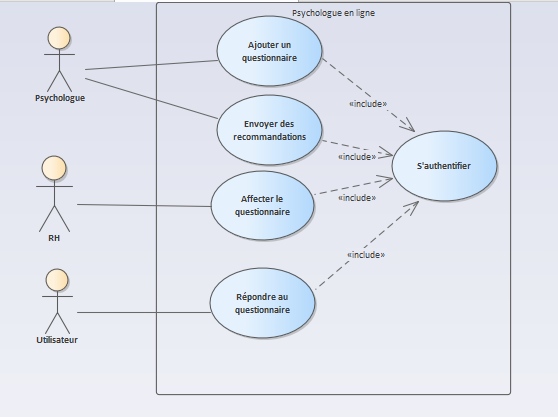
\includegraphics[scale=0.6]{C:/Workplace/Java/project/Capture2.PNG}
\captionof{figure}{Diagramme de cas d'utilisation}
\end{center}
\newpage
\subsection{Description textuelle des principaux cas d'utilisation}
\begin{itemize}

\item Description textuelle du cas d'utilisation "S'authentifier"
\begin{scriptsize}

\begin{tabular}{|l|l|}
\hline
Cas d'utilisation & S'authentifier                                                                                                                                                                                                                                                                                                             \\ \hline
Acteur            & Utilisateur, RH et Psychologue                                                                                                                                                                                                                                                                                             \\ \hline
Objectif          & Permet aux acteurs d'accéder à son propre espace                                                                                                                                                                                                                                                                           \\ \hline
Précondition      & L'acteur doit posséder un  compte                                                                                                                                                                                                                                                                                          \\ \hline
Post condition    & Permet à l'acteur d'accéder à son propre espace                                                                                                                                                                                                                                                                            \\ \hline
Scénario nominal  & \begin{tabular}[c]{@{}l@{}}1-Le système invite l'acteur à entrer son login et son mot de passe.\\ \\ 2-L'acteur saisit le login et le mot de passe.\\ \\ 3-le système vérifie les paramètres.\\ \\ 4-Le système affiche l'espace correspondant à l'acteur.\\ \\ 5-l'instance de cas d'utilisation se termine.\end{tabular} \\ \hline
Exception         & Si un des champs est erroné , le système actualise à nouveau la page                                                                                                                                                                                                                                                       \\ \hline
\end{tabular}
\end{scriptsize}





\item Description textuelle du cas d'utilisation "Ajouter un questionnaire"





\begin{scriptsize}

\begin{tabular}{|l|l|}
\hline
Cas d'utilisation & Ajouter le questionnaire                                                                                                                                                                                                                                                                                                                                                                           \\ \hline
Acteur            & Psychologue                                                                                                                                                                                                                                                                                                                                                                                        \\ \hline
Précondition      & L'acteur accède à l'application                                                                                                                                                                                                                                                                                                                                                                    \\ \hline
Post condition    & Ajouter le questionnaire                                                                                                                                                                                                                                                                                                                                                                           \\ \hline
Scénario nominal  & \begin{tabular}[c]{@{}l@{}}1-Une mappe s'affiche contient la case d'entrer le nom de l'acteur(Psychologue)\\ le choix de sélectionner l'utilisateur une autre case pour rentrer la question \\ et la dernière pour le choix de charger en format CSV.\\ \\ 2-L'acteur rentre les informations suivantes. \\ \\ 3-L'acteur fait envoyer les informations  à l'aide du buttons envoyer.\end{tabular} \\ \hline
Exception         & Pas d'exception                                                                                                                                                                                                                                                                                                                                                                                    \\ \hline
\end{tabular}

\end{scriptsize}


\item Description textuelle du cas d'utilisation "Affecter le questionnaire"

\begin{scriptsize}

\begin{tabular}{|l|l|}
\hline
Cas d'utilisation & Affecter le questionnaire                                                                                                                                                                                                                                                                                                                                  \\ \hline
Acteur            & RH                                                                                                                                                                                                                                                                                                                                                         \\ \hline
Précondition      & L'acteur accède à l'application                                                                                                                                                                                                                                                                                                                            \\ \hline
Post condition    & Approuver le questionnaire                                                                                                                                                                                                                                                                                                                                 \\ \hline
Scénario nominal  & \begin{tabular}[c]{@{}l@{}}1-Une mappe s'affiche contient un tableau des noms des utilisateurs avec \\ leurs psychologues et les états.\\ 2-L'acteur peut approuver le questionnaire par sélectionner oui dans la\\ case état et le rejeter par sélectionner non \\ \\ 3-L'acteur fait envoyer les informations  à l'aide du buttons envoyer.\end{tabular} \\ \hline
Exception         & Pas d'exception                                                                                                                                                                                                                                                                                                                                            \\ \hline
\end{tabular}
\end{scriptsize}

\item Description textuelle du cas d'utilisation "Répondre au questionnaire"




\begin{scriptsize}
\begin{tabular}{|l|l|}
\hline
Cas d'utilisation & Répondre au questionnaire                                                                                                                                                                                                                                                                   \\ \hline
Acteur            & Utilisateur                                                                                                                                                                                                                                                                                 \\ \hline
Précondition      & L'acteur accède à l'application                                                                                                                                                                                                                                                             \\ \hline
Post condition    & Répondre au questionnaire                                                                                                                                                                                                                                                                   \\ \hline
Scénario nominal  & \begin{tabular}[c]{@{}l@{}}1-Une mappe s'affiche contient des questions et une case pour sélectionner\\  le choix\\ 2-L'acteur peut répondre par oui ou non en sélectionnant dans le case\\  répondre\\ 3-L'acteur fait envoyer les informations  à l'aide du buttons envoyer.\end{tabular} \\ \hline
Exception         & Pas d'exception                                                                                                                                                                                                                                                                             \\ \hline
\end{tabular}
\end{scriptsize}

\end{itemize}
\subsection{Conclusion}

 Nous avons essayé tout le long de cette partie de présenter les besoins fonctionnels et non fonctionnels de l'application pour éclaircir et faciliter la compréhension des tâches à réaliser dont le but de faire une conception qui fera l'objet de la partie suivante.





\section{Modélisation conceptuelle}

\subsection{Introduction}

La conception est une étape importante dans la réalisation de l'application. Son objectif principal est de présenter une architecture stable qui permet de définier la réalisation et le fonctionnement du système et aussi éléminer les risques techniques.\\

Pour donner une description abstraite du système, on est intéressé de faire une modélisation de notre application via un diagramme de classe qui va nous offrir une représentation simplifié du système permettant de comprendre et de stimuler ses activités et ses motivations internes.

\subsection{Diagramme de classes}

Nous allons d'abord présenter le diagramme de classe de notre application avec ses éléments.\\

Le diagramme de classes représente la structure statistique d'un système. Il contient les classes , leurs attributs ainsi que leurs associations.\\

L'intéret prinicipal de ce diagramme de classe est de modéliser les entités du système informatique.\\

\subsubsection{Présentation des classes}

Une classe représente la structure d'un objet, la déclaration de l'ensemble des entités qui le composent. Une classe est composée donc de:\\

\begin{itemize}
\item Des attributs : il s'agit des données, dont les valeurs représentent l'état de l'objet.
\item Des méthodes : il s'agit des applications applicables aux objets.
\end{itemize}

Les classes qui forment notre application sont les suivantes:

\begin{itemize}
\item \textbf{Utilisateur:} représente les personnes déjà inscrit dans l'application et qui répond sur le questionnaire ou le formulaire.
\item \textbf{Psychologue:} elle représente l'acteur qui fournit les questions.

\item \textbf{RH:} l'acteur qui approuve  le formulaire.

\item \textbf{Formulaires:} la classe qui contient les informations des utilisateur, les psychologues et les états.

\item \textbf{Questions:} la classe contient les questions et les réponses.

\item \textbf{Notification:}l'entité qui  contient notifications relatives à la réponse des utilisateurs envoyée 
au RH
\item   \textbf{Recommandation:} un objet qui représente une recommandation envoyée pas le psychologue à l'utilisateur
\end{itemize}

\subsubsection{Présentations des attributs et des méthodes}

Les attributs et les méthodes de nos classes sont présentés dans le tableau :


\begin{tabular}{|l|l|l|}
\hline
Nom classe     & La liste des attributs                                                                     & Les méthodes                                                                                                                                                                            \\ \hline
Utilisateur    & \begin{tabular}[c]{@{}l@{}}user\\ mot\_de\_passe\end{tabular}                              & \begin{tabular}[c]{@{}l@{}}getuser()\\ getpasse()\\ authentification()\\ répondre()\end{tabular}                                                                                        \\ \hline
Psychologue    & \begin{tabular}[c]{@{}l@{}}psy\\ mot\_de\_passe\end{tabular}                               & \begin{tabular}[c]{@{}l@{}}getpsy()\\ getpasse()\\ authentification()\\ insérer()\end{tabular}                                                                                          \\ \hline
RH             & \begin{tabular}[c]{@{}l@{}}RH\\ mot\_de\_passe\end{tabular}                                & \begin{tabular}[c]{@{}l@{}}getRH()\\ getpasse()\\ authentification()\\ approuver()\end{tabular}                                                                                         \\ \hline
Formulaires    & \begin{tabular}[c]{@{}l@{}}id\_formulaire\\ utilisateur\\ psychologue\\ etat\end{tabular}  & \begin{tabular}[c]{@{}l@{}}getuser()\\ getpsy()\\ getid\_formulaire()\\ getetat()\\ setuser()\\ setpsy()\\ setetat()\end{tabular}                                                       \\ \hline
Questions      & \begin{tabular}[c]{@{}l@{}}id\_question\\ id\_formulaire\\ question\\ reponse\end{tabular} & \begin{tabular}[c]{@{}l@{}}getid\_question()\\ getid\_formulaire()\\ getquestion()\\ getreponse()\\ setid\_question()\\ setid\_formulaire()\\ setquestion()\\ setreponse()\end{tabular} \\ \hline
notification   & \begin{tabular}[c]{@{}l@{}}id\\ notification\end{tabular}                                  & \begin{tabular}[c]{@{}l@{}}getid()\\ getnotification()\\ envoienotification()\end{tabular}                                                                                              \\ \hline
Recommandation & \begin{tabular}[c]{@{}l@{}}id\\ objet \\ contenuRecommandation\end{tabular}                & \begin{tabular}[c]{@{}l@{}}getid()\\ getobjet()\\ getcontenuRecommandation()\\ setcontenuRecommandation()\\ envoieRocommandation()\end{tabular}                                         \\ \hline
\end{tabular}

\subsubsection{Diagramme de classe}

La figure ci-dessous récapitule le tableau précédent dans un diagramme de classe réalisé à l'aide de l'outil Enterprise Architect et qui englobe toutes les informations qu'on a cité avant:
\begin{center}
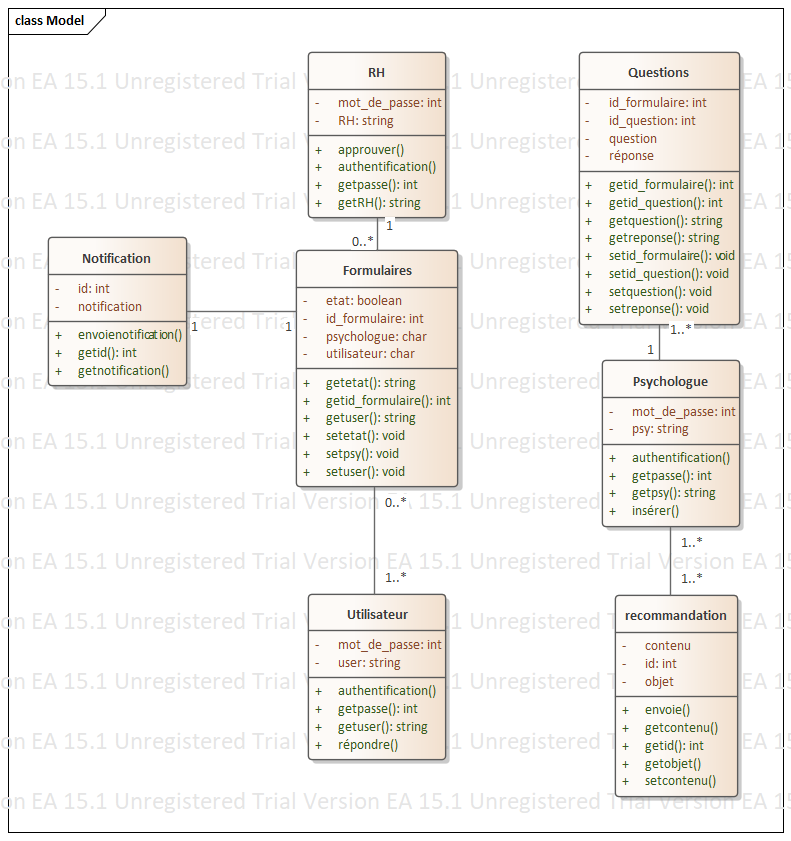
\includegraphics[scale=0.6]{C:/Workplace/java/project/Model.png}
\captionof{figure}{Diagramme de classe}
\end{center}


\newpage




\section{Page Login}
\subsection{Page d'identification}
\indent

Créons premièrement un fichier Login.jsp dans lequel on aura la description de la page d'identification des différents utilisateurs.

\lstset{language=XML}
\begin{scriptsize}
\begin{lstlisting}
<!DOCTYPE html>
<html>
<head>
<meta charset="ISO-8859-1">
<title>Login</title>
</head>
<body>
<div align = "center"> 
 <form action="login" method="post">
  <table>
   <tr>
    <td align ="center">Nom d'utilisateur</td>
   </tr>
   <tr>
    <td><input type="text" name="nom"></td>
   </tr>
   <tr>
    <td align ="center">Mot de passe</td>
   </tr>
   <tr>
    <td><input type="password" nom="mot de passe"></td>
   </tr>
   <tr>
    <td align ="center"><input type="submit" value="Login"></td>
   </tr>
  </table>
 </form>
</div>
</body>
</html>
\end{lstlisting}
\end{scriptsize}
On aura le resultat simple suivant\\

\begin{center}
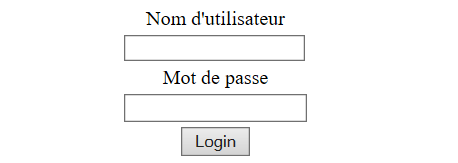
\includegraphics[scale=0.6]{C:/Workplace/java/project/1.png}
\captionof{figure}{Login.jsp}
\end{center}




\subsection{Connexion avec une base de données MySQL : vérification des identifiants}


\subsubsection{Classe Session}
On aura besoin d'une classe \textit{Session} (package : loginsesssion) qui va récupérer pendant chaque identification le nom et le mot de passe entrés.\\

\begin{scriptsize}
\lstset{language=java}
\begin{lstlisting}

package loginsession;

public class session {
	private String nom;
	private String passe;
	public String returnNom() {
		return nom;
	}
	public String affecteNom(String nom) {
		this.nom = nom;
	}
	public String returnPasse() {
		return passe;
	}
	public String affectePasse(String passe) {
		this.passe = passe;
	}
}

\end{lstlisting}
\end{scriptsize}

\subsubsection{Classe DB}

La classe DB (Package : base\_donnees) va permettre dans un premier lieux la connexion avec une base de données MySQL (userdb) qu'on va créer par la suite, puis vérifie si les identifiants (nom et mot de passe) entrés figurent dans cette base.\\

\newpage

\begin{scriptsize}
\lstset{language=java}
\begin{lstlisting}
package base_donnees;
import java.sql.Connection;
import java.sql.DriverManager;
import java.sql.PreparedStatement;
import java.sql.ResultSet;
import java.sql.SQLException;
import loginsession.*;
public class DB {
	private String dbUrl = "jdbc:mysql://localhost:3306/userdb?
                            useJDBCCompliantTimezoneShift=true&
                            useLegacyDatetimeCode=false&serverTimezone=UTC";
	private String dbUname = "AzzimDriouich";
	private String dbPassword = "0000";
	private String dbDriver = "com.mysql.cj.jdbc.Driver";
	public void loadDriver(String dbDriver)
	{
		try {
			Class.forName(dbDriver);
		} catch (ClassNotFoundException e) {
			e.printStackTrace();
		}
	}
	public Connection getConnection()
	{
		Connection con = null;
		try {
			con = DriverManager.getConnection(dbUrl, dbUname, dbPassword);
		} catch (SQLException e) {
			e.printStackTrace();
		}
		return con;
	}
	public boolean valider_donees(Session session)
	{
		boolean status = false;

		loadDriver(dbDriver);
		Connection con = getConnection();
		String sql = "SELECT * 
					  FROM login 
					  WHERE nom = ? 
					  AND mot_de_passe =?";
		PreparedStatement ps;
		try {
		ps = con.prepareStatement(sql);
		ps.setString(1, session.returnNom());
		ps.setString(2, session.returnPasse());
		ResultSet rs = ps.executeQuery();
		status = rs.next();
		
		} catch (SQLException e) {
			e.printStackTrace();
		}
		return status;
	}
}
\end{lstlisting}
\end{scriptsize}


\subsubsection{Création de la base de données "userdb"}


\begin{center}
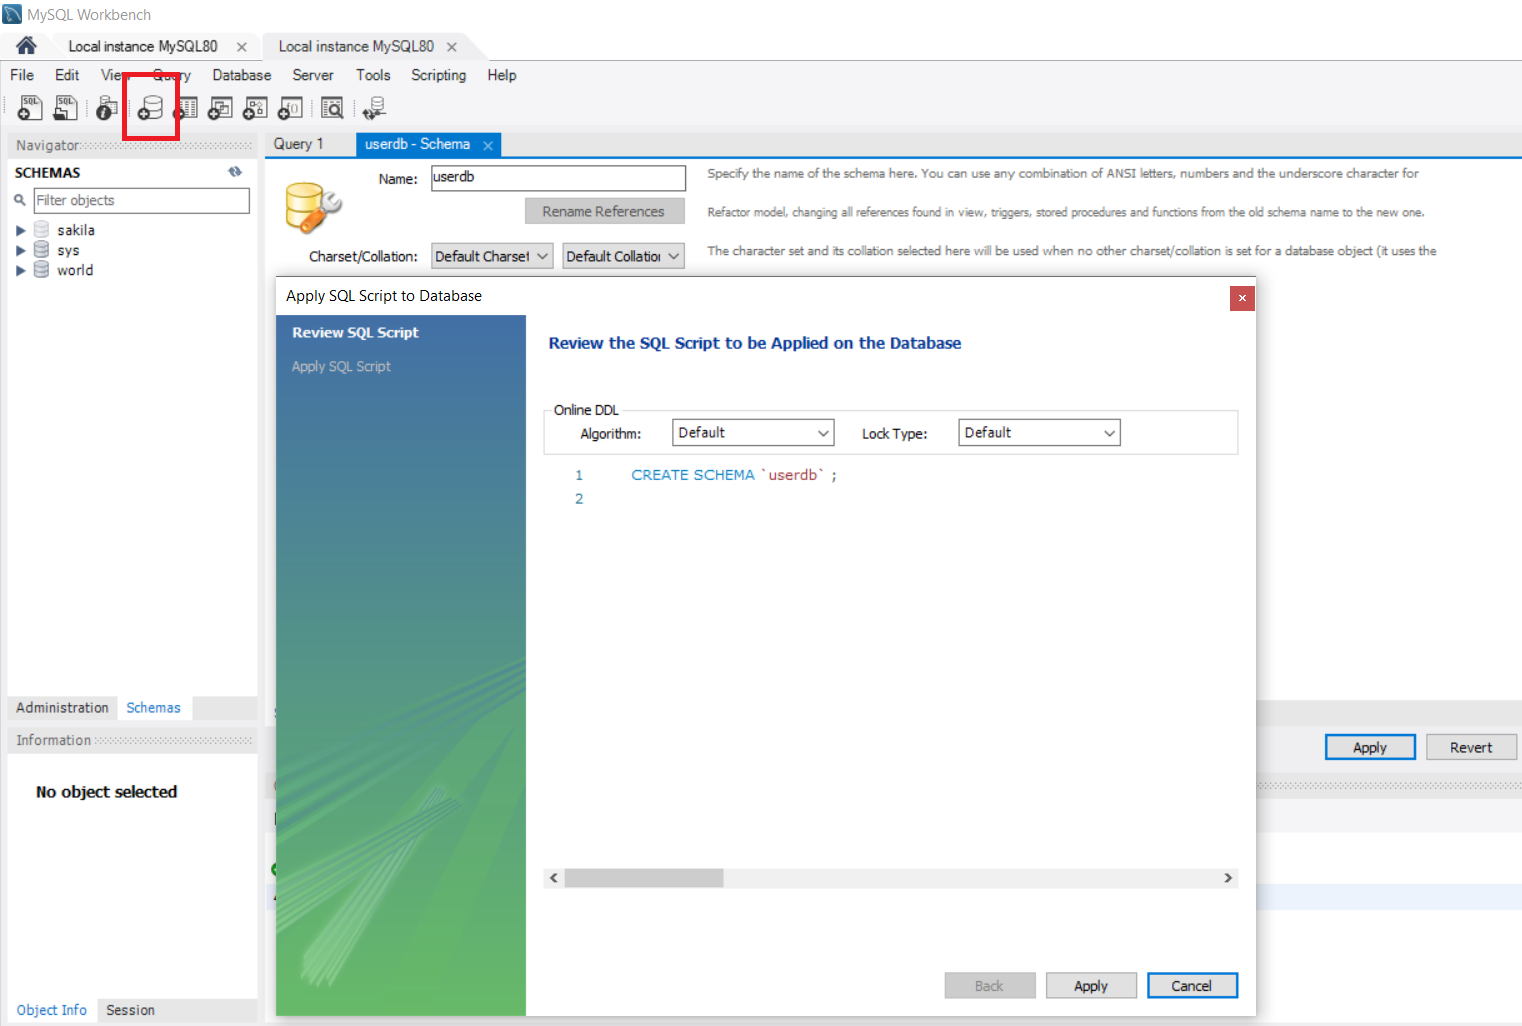
\includegraphics[scale=0.3]{C:/Workplace/java/project/2.png}
\captionof{figure}{create schema}
\end{center}

Après, on doit créer note tableau \textit{login} avec les deux colonnes \textit{nom} (Clé primaire et non null) et \textit{mot\_de\_passe} (non null).\\

\begin{center}
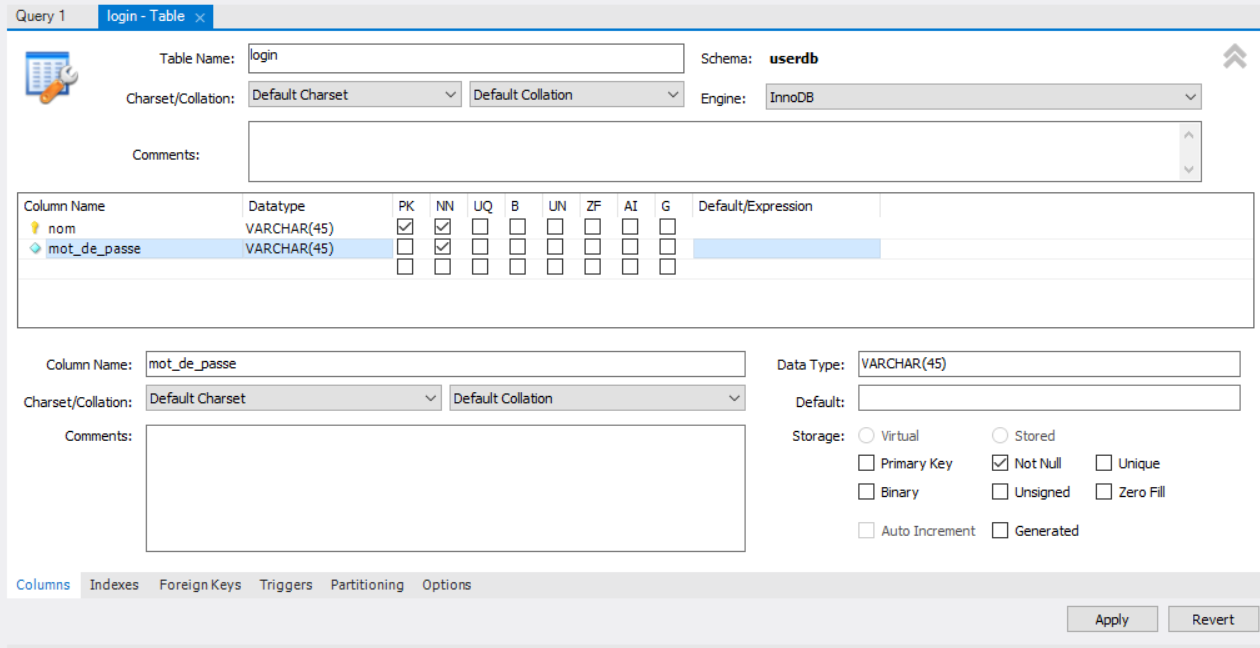
\includegraphics[scale=0.4]{C:/Workplace/java/project/3.png}
\captionof{figure}{Création de la table}
\end{center}

Afin de se connecter, on va insérer quelques utilisateurs à la table \textit{login}.\\


\begin{center}
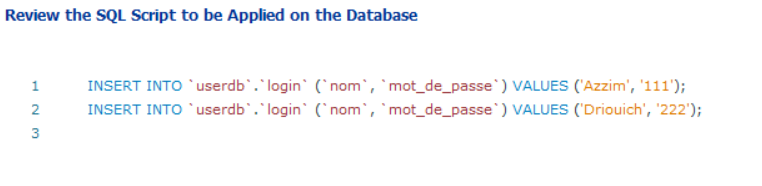
\includegraphics[scale=0.5]{C:/Workplace/java/project/4.png}
\captionof{figure}{Insertion des utilisateurs}
\end{center}






\subsection{Login servlet}

Dans le package web, introduisant la première servlet qui va se servir de l'authentification et diriger l'utilisateur vers sont compte si les identifiants sont corrects ou actualiser la page login sinon.\\

Pour cela, ajoutons un simple fichier Succes.jsp \\


Puis la servlet serait comme suit :\\

\begin{scriptsize}
\lstset{language=java}
\begin{lstlisting}
@WebServlet("/login")
public class LoginServlet extends HttpServlet {
	
	protected void doPost(HttpServletRequest request, 
						  HttpServletResponse response) 
	throws ServletException, IOException {
		String nom = request.getParameter("nom");
		String passe = request.getParameter("mot de passe");
		
	Session session = new Session();
	session.affecteNom(nom);
	session.affectePasse(passe);
	
	DB connexion_db = new DB();
	if(connexion_db.valider_donees(session)) {
		response.sendRedirect("Succes.jsp");
	}
	else {
		response.sendRedirect("login.jsp");
	}
	}
}

\end{lstlisting}
\end{scriptsize}



\subsection{Teste de login}

Exécutons le programme et essayons une authentification avec l'un des utilisateurs déclarés dans la base de données :\\

\begin{center}
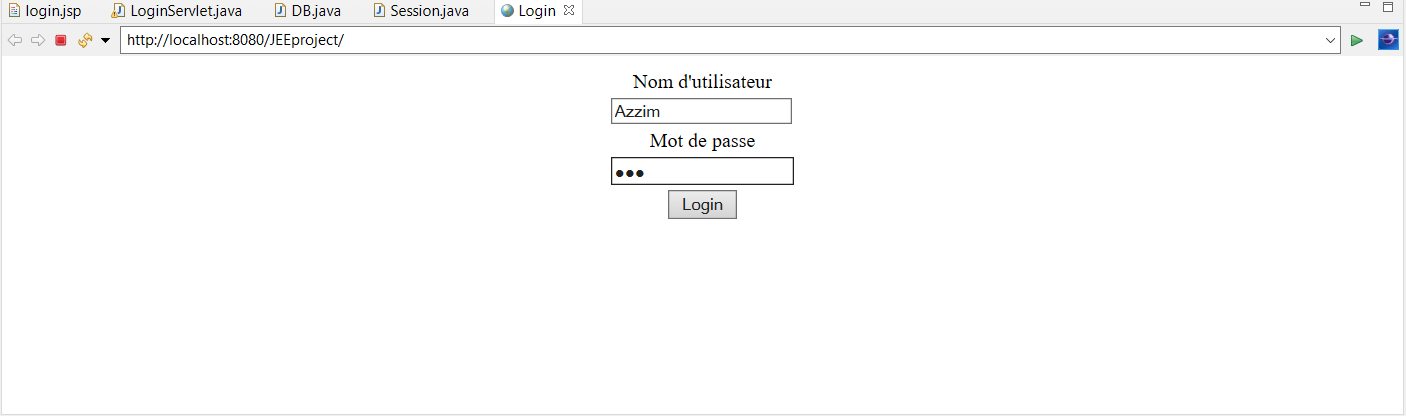
\includegraphics[scale=0.4]{C:/Workplace/java/project/5.png}
\captionof{figure}{Exécution}
\end{center}

\begin{center}
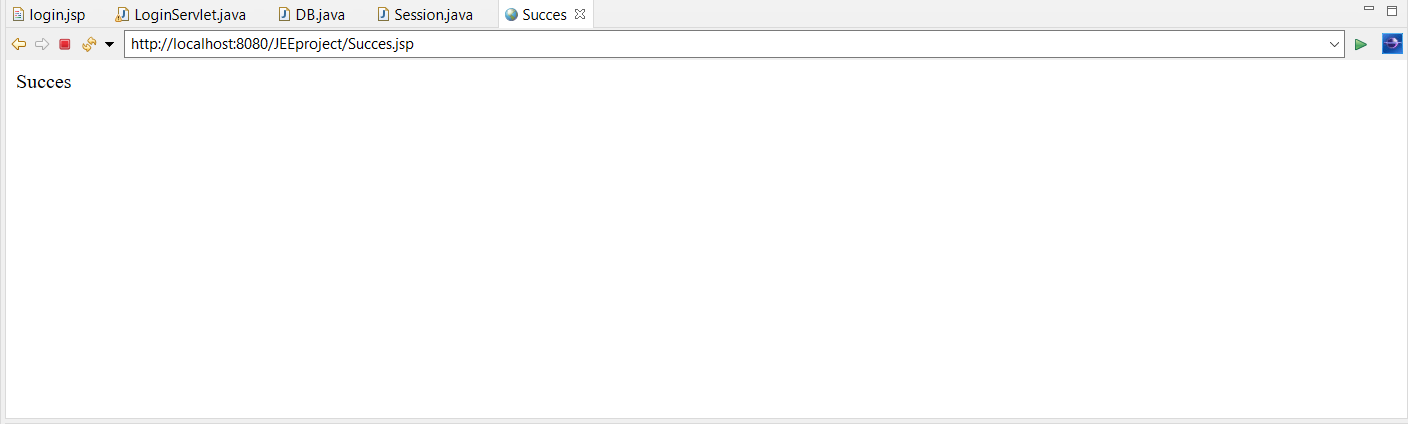
\includegraphics[scale=0.4]{C:/Workplace/java/project/6.png}
\captionof{figure}{Authentification avec succès}
\end{center}


\subsection{Configuration des differents acteurs : Psychologue, RH et Utilisateur }

Après l'authentification, l'inscrit doit être diriger vers sa page personnelle. On distingue entre 3 type d'inscrits : Psychologue, RH et utilisateur. De ce fait, on doit modifier la table \textit{login} en ajoutant la colonne \textit{type}.\\

\begin{center}
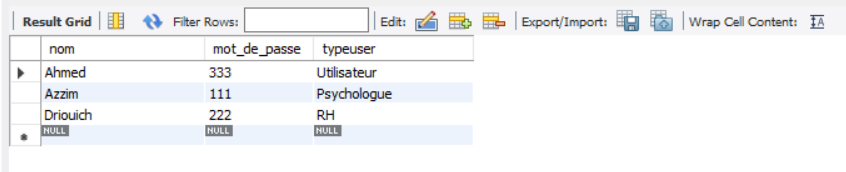
\includegraphics[scale=0.7]{C:/Workplace/java/project/7.png}
\captionof{figure}{Table login}
\end{center}

\newpage

Ensuite on doit modifier la classe \textit{Session} en ajoutant le String type et les méthodes affectType et returnType.\\

\begin{scriptsize}
\lstset{language=java}
\begin{lstlisting}
package loginsession;

public class Session {
	private String nom;
	private String passe;
	private String typeUser;
	public void affectType(String typeUser) {
		this.typeUser = typeUser;
	}
	public String returnType() {
		return typeUser;
	}
	public String returnNom() {
		return nom;
	}
	public void affecteNom(String nom) {
		this.nom = nom;
	}
	public String returnPasse() {
		return passe;
	}
	public void affectePasse(String passe) {
		this.passe = passe;
	}
}

\end{lstlisting}
\end{scriptsize}

\newpage
Pour la classe DB, pendant la validation des identifiants (valide\_donnees), on récupère le type de l'inscrit et on affecte sa valeur à userType en faisant appel à affectType\\



\begin{scriptsize}
\lstset{language=java}
\begin{lstlisting}
public boolean valider_donees(Session session)
{
	boolean status = false;

	loadDriver(dbDriver);
	Connection con = getConnection();
	String sql = "select * from login where nom =? and mot_de_passe =?";
	PreparedStatement ps;
	try {
	ps = con.prepareStatement(sql);
	ps.setString(1, session.returnNom());
	ps.setString(2, session.returnPasse());
	ResultSet rs = ps.executeQuery();
	status = rs.next();
	session.affectType(rs.getString("typeuser"));
	} catch (SQLException e) {
		e.printStackTrace();
	}
	return status;
}
\end{lstlisting}
\end{scriptsize}

\newpage

Finalement la servlet doit diriger chaque type d'inscrit vers sa page personnelle (Psychologue.jsp, RH.jsp ou Utilisateur.jsp)\\

\begin{scriptsize}
\lstset{language=java}
\begin{lstlisting}
@WebServlet("/login")
public class LoginServlet extends HttpServlet {
	
	protected void doPost(HttpServletRequest request, 
						  HttpServletResponse response) 
	throws ServletException, IOException {
		String nom = request.getParameter("nom");
		String passe = request.getParameter("mot de passe");
		
	Session session = new Session();
	session.affecteNom(nom);
	session.affectePasse(passe);
	DB connexion_db = new DB();
	if(connexion_db.valider_donees(session)) {
		if(session.returnType().equals("Psychologue")) {
			response.sendRedirect("Psychologue.jsp");
		}
		else if(session.returnType().equals("Utilisateur")) {
			response.sendRedirect("Utilisateur.jsp");
		}
		else if(session.returnType().equals("RH")) {
			response.sendRedirect("RH.jsp");
		}
	}
	else {
		response.sendRedirect("login.jsp");
	}
	}

}
\end{lstlisting}
\end{scriptsize}


\subsection{Partie CSS}

Pour finir cette partie, introduisant un fichier css \textit{loginCSS.css} pour les raisons esthétiques.\\


\begin{scriptsize}

\lstset{language=CSS}
\begin{lstlisting}
button {
  background-color: while;
  color: black;
  padding: 14px 20px;
  border-radius: 10px;
  margin: 8px 0;
  border: none;
  cursor: pointer;
  width: 100%;
}
input[type=text], input[type=password] {
  width: 100%;
  border-radius: 10px;
  padding: 12px 20px;
  margin: 8px 0;
  display: inline-block;
  border: 1px solid #ccc;
  box-sizing: border-box;
}
button:hover {
  opacity: 0.8;
  background-color: black;
  color: white;
}
body {
 background-image: url("1.gif");
 background-attachment: fixed;
 background-repeat: no-repeat;
 background-position: center;
 background-size: cover;
 background-color: white;
}

.login {
  overflow: hidden;
  opacity: 0.8;
  background-color: #8e8e8e;
  padding: 20px 30px 30px 30px;
  border-radius: 10px;
  top:100px;
  width: 400px;
  box-shadow: 5px 10px 10px rgba(green, 0.2);
}

\end{lstlisting}
\end{scriptsize}



le fichier \textit{login.jsp} sera aussi changé 


\lstset{language=XML}
\begin{scriptsize}
\begin{lstlisting}
<!DOCTYPE html>
<html>
<head>
<meta charset="ISO-8859-1">
<title>Login</title>
</head>
<link href="loginCSS.css" rel="stylesheet" type="text/css"><body>
<div align = "center">
 <form class = login action="login" method="post">
  <table>
   <tr>
    <td><input type="text" name="nom" placeholder="Nom d'utilisateur"></td>
   </tr>
   <tr>
    <td><input type="password" name="mot de passe" placeholder="Password"></td>
   </tr>
   <tr>
    <td align ="center"><button type="submit" value="Login">login</button></td>
   </tr>
  </table>
 </form>
</div>
</body>
</html>
\end{lstlisting}
\end{scriptsize}


Résultat final :

\begin{center}
\hspace*{-2cm}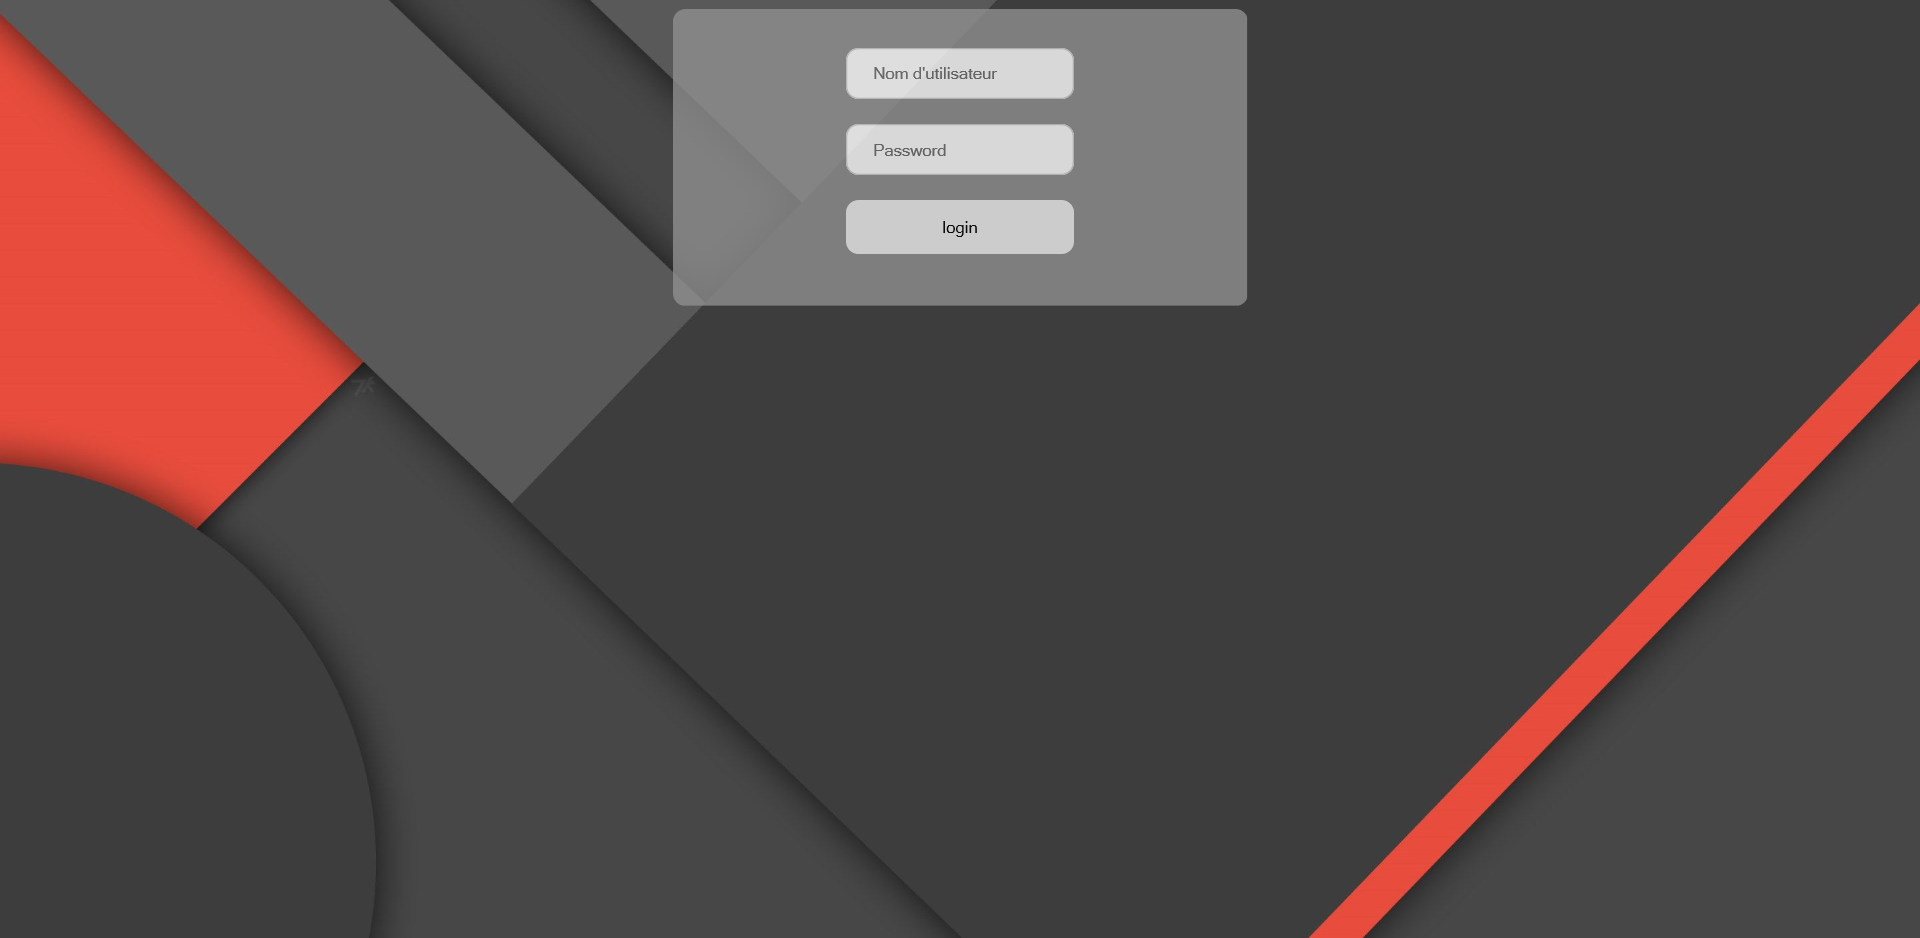
\includegraphics[scale=0.4]{C:/Workplace/java/project/14.png}
\captionof{figure}{Page login}
\end{center}














\section{Conception de la base de données}

De plus du tableau \textit{login} on aura besoin d'autres pour stocker les questions posés par les psychologues et les réponses récupérés de la part des utilisateurs.\\
On propose l'ajout de deux tableaux :\\
\begin{itemize}
\item Formulaires : renferme l'id du formulaire (Clé primaire), le nom du psychologue ( Créateur du formulaire ), le nom d'utilisateur ( Destinataire ) et l'état du formulaire ( Approuvé ou non par le RH ).\\
\item Questions : contient la question, son l'id ( Clé primaire ), l'id du formulaire où se trouve et les réponses fournies par les utilisateurs.
\end{itemize}


\begin{center}

\begin{tabular}{|c|c|c|c|}
\hline
\multicolumn{4}{|c|}{\textbf{Formulaires}}                                                                                                                                                                                                        \\ \hline
\textbf{id\_formulaire}                                    & \textbf{utilisateur}                                       & \textbf{psychologue}                                       & \textbf{etat}                                              \\ \hline
\textbf{\begin{tabular}[c]{@{}c@{}}.\\ .\\ .\end{tabular}} & \textbf{\begin{tabular}[c]{@{}c@{}}.\\ .\\ .\end{tabular}} & \textbf{\begin{tabular}[c]{@{}c@{}}.\\ .\\ .\end{tabular}} & \textbf{\begin{tabular}[c]{@{}c@{}}.\\ .\\ .\end{tabular}} \\ \hline
\end{tabular}



\begin{tabular}{|c|c|c|c|}
\hline
\multicolumn{4}{|c|}{\textbf{Questions}}                                                                                                                                                                                                          \\ \hline
\textbf{id\_question}                                      & \textbf{question}                                    & \textbf{id\_formulaire}                                          & \textbf{reponse}                                           \\ \hline
\textbf{\begin{tabular}[c]{@{}c@{}}.\\ .\\ .\end{tabular}} & \textbf{\begin{tabular}[c]{@{}c@{}}.\\ .\\ .\end{tabular}} & \textbf{\begin{tabular}[c]{@{}c@{}}.\\ .\\ .\end{tabular}} & \textbf{\begin{tabular}[c]{@{}c@{}}.\\ .\\ .\end{tabular}} \\ \hline
\end{tabular}
\end{center}


La création des deux tableaux consiste à lancer les deux requêtes :\\



\begin{center}
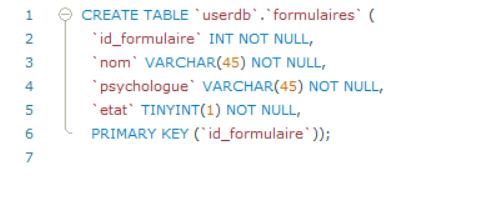
\includegraphics[scale=0.7]{C:/Workplace/java/project/15.png}
\captionof{figure}{table formulaires}

\vspace{1cm}
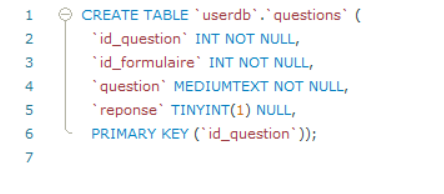
\includegraphics[scale=0.7]{C:/Workplace/java/project/16.png}
\captionof{figure}{table questions}
\end{center}


Insérant par suite quelques données dans les tables pour qu'elles nous aident pendant la construction des interfaces des utilisateurs (formulaire 101 avec 2 questions 201 et 202 et formulaire 102 avec une question 203)\\

 



\begin{center}
\hspace*{-2cm}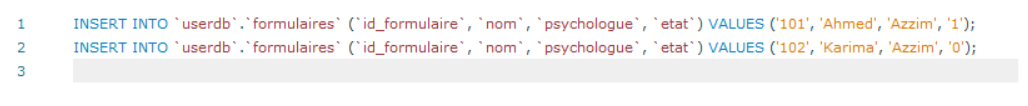
\includegraphics[scale=0.7]{C:/Workplace/java/project/17.png}
\captionof{figure}{table formulaires}

\vspace{1cm}
\hspace*{-3cm}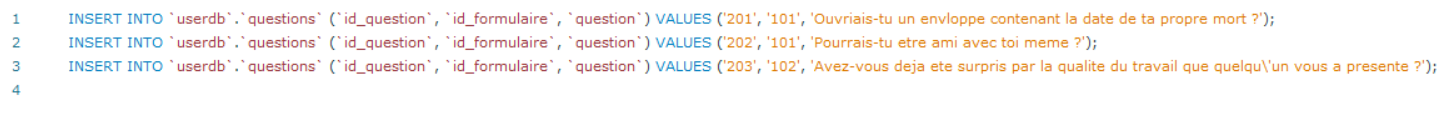
\includegraphics[scale=0.6]{C:/Workplace/java/project/18.png}
\captionof{figure}{table questions}
\end{center}


Maintenant que tout est prêt, construisons les interfaces des utilisateurs.\\

\section{Interface "Utilisateur"}
\indent


L'utilisateur doit être capable de voir les questions du formulaire fournit par le psychologue et approuvé par le RH. Il doit aussi avoir le droit de répondre à chaque question avec oui ou non. Finalement, il confirme ses réponses pour qu'elles soient envoyés au psychologue.\\
\subsection{Classe Question}

La première étape consiste à créer une classe \textit{Question} (Similaire à \textit{Session}) dont les attributs sont les colonnes du tableau Questions. \\




\begin{scriptsize}

\lstset{language=java}
\begin{lstlisting}
package loginsession;

public class Question {
	public int id_question;
	public int id_formulaire;
	public String questiontext;
	public boolean reponse;
	
	public void affectIdQuestion(int id_question) {
		this.id_question =id_question;
	}
	public int returnIdQuestion() {
		return id_question;
	}
	public void affectIdFormulaire(int id_formulaire) {
		this.id_formulaire =id_formulaire;
	}
	public int returnIdformulaire() {
		return id_formulaire;
	}
	public String returnQuestion() {
		return questiontext;
	}
	public void affectQuestion(String questiontext) {
		this.questiontext = questiontext;
	}
	public boolean returnReponse() {
		return reponse;
	}
	public void affectReponse(boolean reponse) {
		this.reponse =reponse;
	}
	
}
\end{lstlisting}

\end{scriptsize}

\subsection{Chargement des questions depuis la base de données}

Ensuite, on déclare la fonction question\_utilisateur() qui prend en argument une \textit{Session} et une liste des objets de la classe \textit{Question} puis ajoute dans cette liste les questions du formulaire envoyé à cet utilisateur et qui sont approuvés par le RH.\\


Le tableau désiré est résultat de la requête :\\
\textbf{SELECT} * \\
\textbf{FROM} userdb.questions q \\
\textbf{INNER JOIN} userdb.formulaires f \\
\textbf{ON} f.id\_formulaire = q.id\_formulaire\\
\textbf{WHERE} f.nom=? \\
\textbf{AND} f.etat=1\\

Le champ f.nom serait remplis par session.nom.



\begin{scriptsize}
\lstset{language=java}
\begin{lstlisting}
public void question_utilisateur(Session session, List<Question> userquestion)
	{
		boolean status;

		loadDriver(dbDriver);
		Connection con = getConnection();
		String sql = "SELECT * FROM userdb.questions q 
					  INNER JOIN userdb.formulaires f 
					  ON f.id_formulaire=q.id_formulaire 
					  WHERE f.nom=? AND f.etat=1";
		PreparedStatement ps;
		try {
		ps = con.prepareStatement(sql);
		ps.setString(1, session.returnNom());
		ResultSet rs = ps.executeQuery();
		status = rs.next();
		while(status) {
			Question question = new Question();
			question.affectIdQuestion(rs.getInt("id_question"));
			question.affectIdFormulaire(rs.getInt("id_formulaire"));
			question.affectReponse(rs.getBoolean("reponse"));
			question.affectQuestion(rs.getString("question"));

			userquestion.add(question);
			status = rs.next();
		}
		} catch (SQLException e) {
			e.printStackTrace();
		}
	}
\end{lstlisting}

\end{scriptsize}



\subsection{Affichage des questions}

Finalement, dans la partie \emph{Utilisateur} de la servlet, on introduit la liste \textit{userquestion} des objets de la classe \textit{Question} qui serait remplies par la fonction \textit{question\_utilisateur()} et envoyée vers Utilisateur.jsp.


\begin{scriptsize}
\lstset{language=java}
\begin{lstlisting}
else if(session.returnType().equals("Utilisateur")) {
	List<Question> userquestion = new ArrayList<Question>();
	connexion_db.question_utilisateur(session, userquestion);
	request.setAttribute("userquestion", userquestion);
	request.setAttribute("utilisateur", session.returnNom());
	RequestDispatcher rst = request.getRequestDispatcher("Utilisateur.jsp");
	rst.forward(request, response);
		}
\end{lstlisting}

\end{scriptsize}


Finalement, la liste des questions peut être affichée à l'aide de foreach.\\

\begin{scriptsize}
\lstset{language=XML}
\begin{lstlisting}
<%@page contentType="text/html" pageEncoding="UTF-8"%>
<%@taglib uri="http://java.sun.com/jsp/jstl/core" prefix="c"%>
<!DOCTYPE html>
<html>
<head>
<meta charset="UTF-8">
<title>${utilisateur}</title>

</head>
<link href="UtilisateurCSS.css" rel="stylesheet" type="text/css">
<body>
 <form class=envoie action="envoie" method="post">
  <br>
  <br>
  <h1 align=center>Veuillez repondre aux questions suivantes</h1>
  <br>
  <br>
  <div class="container">
   <table align=center>
    <thead>
     <tr>
      <th>Question</th>
      <th>Reponse</th>
     </tr>
    </thead>
    <tbody>
     <c:forEach items="${userquestion}" var="question">
      <tr>
       <td><c:out value="${question.returnQuestion()}" /></td>
       <td>
        <select name="reponse" class="dropbtn">
         <option value="false">Oui</option>
         <option value="true">Non</option>
        </select></td>
      </tr>
     </c:forEach>
    </tbody>
    <thead>
     <tr>
      <td></td>
      <th align=center><button type="submit" value="Login">Envoyer</button></th>
     </tr>
    </thead>
   </table>
  </div>
 </form>
</body>
</html>
\end{lstlisting}

\end{scriptsize}


\subsection{Partie CSS}

Le fichier CSS décrivant la page utilisateur est donné par : 


\begin{scriptsize}

\lstset{language=CSS}
\begin{lstlisting}
@import url(https://fonts.googleapis.com/css?family=Open+Sans:400,600);
h1{
	 font-size: 20px;
	 font-family: 'Courier New';
	 color : white;
}
button {
  background-color: white;
  color: black;
  display:inline-block;
  padding: 10px 30px;
  border-radius: 10px;
  font-size: 20px;
  margin: 30px 0;
  border: none;
  cursor: pointer;
  display: inline-block;
  transition: all 0.25s;
}

button:hover {
  opacity: 0.8;
  background-color: #E2B842;
  color: white;
}

*, *:before, *:after {
  margin: 0;
  padding: 0;
  box-sizing: border-box;
}
.dropbtn {
  background-color: #012B39;
  color: #ffffff;
  padding: 10px 30px;
  font-size: 15px;
  border: none;
  cursor: pointer;
}
body {
  background: #105469;
  font-family: 'Open Sans', sans-serif;
}
table {
  width: 70%;
  background: #012B39;
  border-radius: 0.25em;
  border-collapse: collapse;
  margin: 1em;
}
th {
  border-bottom: 1px solid #364043;
  color: #E2B842;
  font-size: 20px;
  font-weight: 600;
  padding: 0.5em 1em;
  text-align: Left;
}
td {
  color: #fff;
  font-weight: 400;
  padding: 0.65em 1em;
}
.disabled td {
  color: #4F5F64;
}
tbody tr {
  transition: background 0.25s ease;
}
tbody tr:hover {
  background: #014055;
}
\end{lstlisting}
\end{scriptsize}


Résultat donné pour utilisateur "Ahmed" :\\

\begin{center}
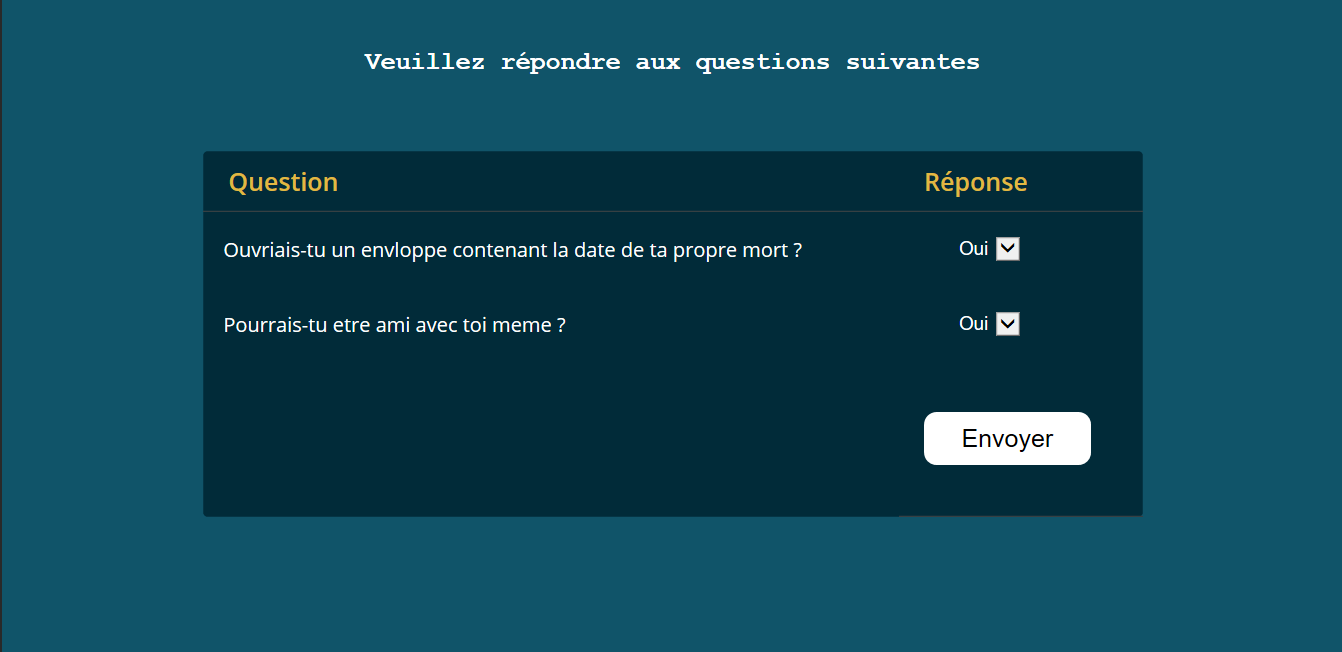
\includegraphics[scale=0.5]{C:/Workplace/java/project/19.png}
\captionof{figure}{Interface utilisateur}
\end{center}

\section{Interface "RH"}

Un RH doit être capable de voir les noms des utilisteurs accompagnés par les noms des psycholoques
pour les approuver ou les rejetter. 
\subsection{Classe Formulaire}

Dans un premier pas on va créer une classe Formulaire dont les attributs sont les colonnes du tableau formulaires.
\begin{scriptsize}

\lstset{language=java}
\begin{lstlisting}
package loginsession;

public class Formulaire {
	public int id_formulaire;
	public String nom;
	public String psychologue;
	public boolean etat;
	
	public String getuser() {
		return nom;}
		
	public void setuser(String nom) {
	        this.nom = nom;
	    }
	public String getpsy() {
	        return psychologue;
	    }
	 public void setpsy(String psychologue) {
	        this.psychologue = psychologue;
	    }
    public boolean returnetat() {
			return etat;
		}
    public void affectetat(boolean etat) {
			this.etat =etat;
		}
}
\end{lstlisting}
\end{scriptsize}
\subsection{Chargement des formulaires depuis la base de donnée}

On déclare la fonction liste\_formulaire() qui prend en argument deux paramètres \textit{Session} et \textit{liste des Objets de la classe Formulaire} puis il rajoute dans cette l'approuvement ou le rejet du RH.

\begin{scriptsize}
\lstset{language=java}
\begin{lstlisting}
public void liste_formulaire(Session session, List<Formulaire> RH) {
        Statement statement = null;
        ResultSet resultat = null;

        loadDriver(dbDriver);
        Connection connexion = getConnection();
        try {
            statement = connexion.createStatement();
            resultat = statement.executeQuery("SELECT * FROM userdb.formulaires;");
            while (resultat.next()) {
                String user = resultat.getString("nom");
                String psy = resultat.getString("psychologue");
                boolean etat = resultat.getBoolean("etat");
                Formulaire formulaire = new Formulaire();
                formulaire.setuser(user);
                formulaire.affectetat(etat);
                formulaire.setpsy(psy);
                RH.add(formulaire);
                System.out.println(user);           }
        } catch (SQLException e) {
          e.printStackTrace();
            
        }
       
    }
\end{lstlisting}
\end{scriptsize}

\subsection{Affichage de formulaire}

Finalement, on fait un autre changement dans la partie RH de la servlet, on introduit la liste RH des objets de la classe \textit{Formulaire} qui serait remplie par la fonction \textit{liste\_formulaire()} et envoyée vers RH.jsp.
\begin{scriptsize}

\lstset{language=java}
\begin{lstlisting}
 else if(session.returnType().equals("RH")) {
	List<Formulaire> RH = new ArrayList<Formulaire>();
	connexion_db.liste_formulaire(session,RH);
	request.setAttribute("RH", RH);
	RequestDispatcher rst = request.getRequestDispatcher("RH.jsp");
	rst.forward(request, response);
     }
\end{lstlisting}
\end{scriptsize}


Maintenant pour le fichier JSP ,la liste des utilisateurs et des psychologues est affichée par foreach.
\begin{scriptsize}

\lstset{language=XML}
\begin{lstlisting}
<%@page contentType="text/html" pageEncoding="UTF-8"%>
<%@taglib uri="http://java.sun.com/jsp/jstl/core" prefix="c"%>
<!DOCTYPE html>
<html>
<head>
<meta charset="UTF-8">
<title>${formulaire}</title>

</head>
<link href="RHCSS.css" rel="stylesheet" type="text/css">
<body>
 <form class=envoie action="envoie" method="post">
  <br>
  <br>
  <h1 align=center>Veuillez approuver les etats suivants</h1>
  <br>
  <br>
  <div class="container">
   <table align=center>
    <thead>
     <tr>
      <th>Utilisateur</th>
      <th>Psychologue</th>
      <th>l'etat</th>
     </tr>
    </thead>
    <tbody>
     <c:forEach items="${RH}" var="formulaire">
      <tr>
       <td><c:out value="${formulaire.getuser()}" /></td>
       <td><c:out value="${formulaire.getpsy()}" /></td>
       <td>
        <select name="etat" class="dropbtn">
         <option value="false">Non</option>
         <option value="true">Oui</option>
        </select></td>
      </tr>
     </c:forEach>
    </tbody>
    <thead>
     <tr>
      <td></td>
      <th align=center><button type="submit" value="Login">Envoyer</button></th>
     </tr>
    </thead>
   </table>
  </div>
 </form>
</body>
</html>

\end{lstlisting}
\end{scriptsize}
 
\subsection{Partie CSS}
Le fichier CSS décrivant la page RH est celui de l'utilisateur.

On obtient le résultat suivant:

\begin{center}
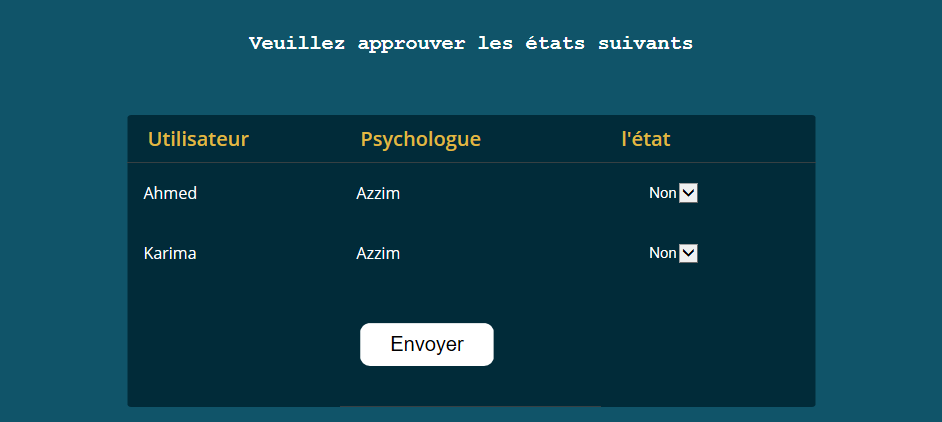
\includegraphics[scale=0.5]{C:/Workplace/Java/project/Capture.PNG}
\captionof{figure}{Interface RH}
\end{center}




\newpage









\section{Interface "Psychologue"}

\subsection{Affichage des formulaires}

Un psychologue doit être capable de voir les réponses de ses patients aux formulaires crées. Si le formulaire n'est pas encore approuvé par le RH ou respectivement le patient n'a pas encore répondu, le message 'PAS ENCORE APPROUVE' respectivement 'EN ATTENTE' doivent êtres affichés.\\
Définissons dans un premier temps les deux fonctions :\\
\begin{itemize}
\item liste\_formulaire\_psychologue() qui prend en argument le nom du psychologue et une liste des objets de la classe \textit{Formulaire} puis ajoute à cette liste les formulaires récupérés par la requête :\\

\begin{scriptsize}
\textbf{SELECT} * \textbf{FROM} userdb.formulaires f \textbf{WHERE} f.psychologue = ?
\end{scriptsize}

\begin{scriptsize}

\begin{lstlisting}
public void liste_formulaire_psychologue(String nom, List<Formulaire> formulaires) {

	loadDriver(dbDriver);
	PreparedStatement ps;
	Connection con = getConnection();
	String sql = "SELECT * FROM userdb.formulaires f where f.psychologue = ?";

	try {
		ps = con.prepareStatement(sql);
		ps.setString(1, nom);
		ResultSet resultat = ps.executeQuery();
		while (resultat.next()) {
			String user = resultat.getString("nom");
			String psy = resultat.getString("psychologue");
			boolean etat = resultat.getBoolean("etat");
			int id_formulaire = resultat.getInt("id_formulaire");
			Formulaire formulaire = new Formulaire();
			formulaire.setuser(user);
			formulaire.affectetat(etat);
			formulaire.setpsy(psy);
			formulaire.affectIdFormulaire(id_formulaire);
			formulaires.add(formulaire);
		}
	} catch (SQLException e) {
		e.printStackTrace();
	}
}
\end{lstlisting}



\end{scriptsize}





\item question\_utilisateur\_psychologue() qui prend en argument le nom de l'utilisateur et une liste des objets de la classe \textit{Question} puis ajoute à cette liste les questions récupérés par la requête :\\\\
\begin{scriptsize}
\textbf{SELECT} * \textbf{FROM} userdb.questions q \\
\textbf{INNER JOIN} userdb.formulaires f \\
\textbf{ON} f.id\_formulaire=q.id\_formulaire \textbf{WHERE} f.nom=?
\end{scriptsize}

\end{itemize}


\begin{scriptsize}
\begin{lstlisting}
public void question_utilisateur_psychologue(String Psychologue,
											 List<Question> userquestion) {
	boolean status;

	loadDriver(dbDriver);
	Connection con = getConnection();
	String sql = "SELECT * FROM userdb.questions q 
				  INNER JOIN userdb.formulaires f 
				  ON f.id_formulaire=q.id_formulaire WHERE f.nom=?";
	PreparedStatement ps;
	try {
		ps = con.prepareStatement(sql);
		ps.setString(1, Psychologue);
		ResultSet rs = ps.executeQuery();
		status = rs.next();
		while (status) {
			Question question = new Question();
			question.affectIdQuestion(rs.getInt("id_question"));
			question.affectIdFormulaire(rs.getInt("id_formulaire"));
			question.affectReponse(rs.getBoolean("reponse"));
			question.affectQuestion(rs.getString("question"));
			question.affectEtatQuestion(rs.getString("reponse"));
			userquestion.add(question);
			status = rs.next();
		}
	} catch (SQLException e) {
		e.printStackTrace();
	}
}

\end{lstlisting}
\end{scriptsize}



\newpage

Ensuite dans la servlet login, au cas ou le type l'utilisateur identifié est de type psychologue on exécute les lignes si dessous

\begin{scriptsize}
\begin{lstlisting}
if (session.returnType().equals("Psychologue")) {
	List<Formulaire> formulaires = new ArrayList<Formulaire>();
	List<Question> userquestion = new ArrayList<Question>();
	
	connexion_db.liste_formulaire_psychologue(session.returnNom(), formulaires);
	connexion_db.question_utilisateur_psychologue(session.returnNom(), userquestion);
	
	request.setAttribute("psy", session.returnNom());
	request.setAttribute("userquestion", userquestion);
	request.setAttribute("formulaires", formulaires);
	RequestDispatcher rst = request.getRequestDispatcher("Psychologue.jsp");
	rst.forward(request, response);
\end{lstlisting}
\end{scriptsize}



Le reste du travaille serait dans le fichier Psychologue.jsp :\\
Le premier attribue "psy" contenant le nom du psychologue serait la valeur d'une input de type caché car on se servira d'elle dans la création des formulaires.\\

A l'aide des 2 listes (userquestion et formulaires) envoyées vers ce fichier, on doit assurer un affichage des questions et leurs états.\\

Pour chaque formulaire, une table est crée ( foreach ligne 19 )  puis pour chaque table on affichera que les questions qui appartient à ce formulaire ( test if en ligne 30 ).\\

Finalement la colonne réponse assurera les états des questions :
\begin{enumerate}
\item Si le formulaire est approuvé par le RH ( ligne 38 ) on aura deux cas
\begin{itemize}
\item Le patient n'a pas encore répondu ( ligne 40 ), on affichera "EN ATTENTE".
\item Le patient a répondu, on affichera la réponse ( ligne 44 ).
\end{itemize} 
\item Sinon, le RH n'a pas encore approuvé ( ligne 48 ) on affichera "PAS ENCORE APPROUVE"
\end{enumerate}


\newpage




\begin{scriptsize}
\lstset{language=XML}
\begin{lstlisting}
<%@page contentType="text/html" pageEncoding="UTF-8"%>
<%@taglib uri="http://java.sun.com/jsp/jstl/core" prefix="c"%>
<!DOCTYPE html>
<html>
<head>
<meta charset="ISO-8859-1">
<input type="hidden" name="Psychologue" value="${psy}" />
<title>Psychologue ${psy}</title>
</head>
<link href="UtilisateurCSS.css" rel="stylesheet" type="text/css">
<body>
 <br>
 <form action="NouveauFormulaire" method="post">
 <h1 align="center">
  <button type="submit">Nouveau formulaire</button>
 </h1>
 <input type="hidden" name="Psychologue" value="${psy}" />
 </form>
 <c:forEach items="${formulaires}" var="formulaire">
  <div class="container">
   <table align="center">
    <thead>
     <tr>
      <th><c:out value="${formulaire.getuser()}" /></th>
      <th>reponses</th>
     </tr>
    </thead>
    <tbody>
     <c:forEach items="${userquestion}" var="question">
     <c:if test="${question.returnIdformulaire() == formulaire.returnIdFormulaire()}">
      <tr>
       <td>
        <c:out value="${question.returnQuestion()}" />
       </td>
       <input type="hidden" name="idQuestion" value="${question.returnIdQuestion()}" />
       <td>
        <c:choose>	
         <c:when test="${formulaire.returnetat()}">
          <c:choose>
		   <c:when test="${question.returnEtatQuestion() == null}">
			<c:out value = "EN ATTENTE"/>
		   </c:when>
		   <c:otherwise>
			<c:out value="${question.returnReponse() ? 'Oui':'Non'}"/>
		   </c:otherwise>
		  </c:choose>
		 </c:when>
   		 <c:otherwise>
		  <c:out value="PAS ENCORE APPROUVE"/>
		 </c:otherwise>
		</c:choose>
	   </td>
	   </tr>
	  </c:if>
	 </c:forEach>
	</tbody>
   </table>
  </div>
 </c:forEach>
</body>
</html>
\end{lstlisting}
\end{scriptsize}




Un exemple de résultat :


\begin{center}
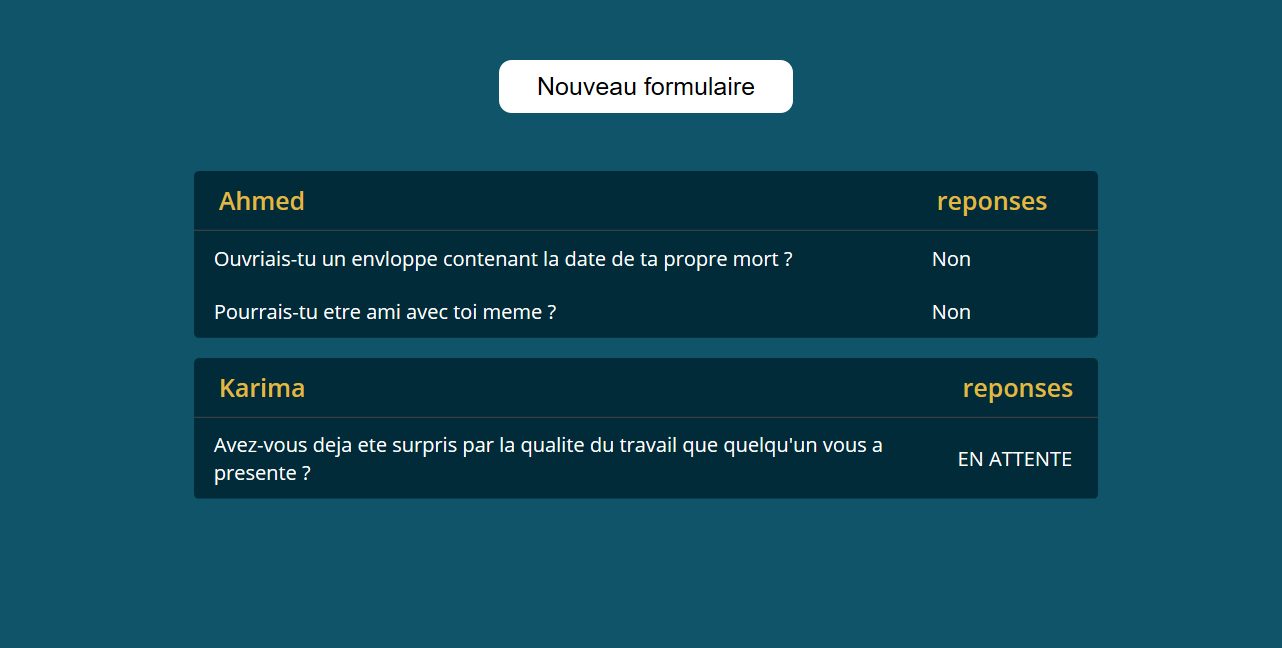
\includegraphics[scale=0.4]{C:/Workplace/Java/project/25.PNG}
\captionof{figure}{Interface Psychologue}
\end{center}



\subsection{Création des formulaires}



Le bouton "Nouveau formulaire" doit rediriger le psychologue vers une autre page dans laquelle il peut construire ses propres formulaires.\\

La première tache consiste a choisir le destinataire. De ce fait, on définit la fonction liste\_destinataires() (Classe DB) qui retourne l'ensemble des utilisateurs existant dans la base de données.
\newpage



\begin{scriptsize}
\lstset{language=java}
\begin{lstlisting}
public List<String> liste_destinataires() {
	List<String> liste = new ArrayList<String>();
	loadDriver(dbDriver);
	PreparedStatement ps;
	Connection con = getConnection();
	String sql = "SELECT * FROM userdb.login l Where l.typeuser = 'Utilisateur'";
	try {
		ps = con.prepareStatement(sql);
		ResultSet rst = ps.executeQuery();
		while (rst.next()) {
			String user = rst.getString("nom");
			liste.add(user);
		}
	} catch (SQLException e) {
		e.printStackTrace();
	}

	return liste;
}
\end{lstlisting}
\end{scriptsize}



Puis une autre fonction EntrerFormulaireEtQuestions() qui prend en argument le nom du psychologue, le nom de l'utilisateur et une liste des questions puis insère dans la base de données un nouveau formulaire dans la table "Formulaires" et la liste des question dans la table "Questions".\\

Avant l'insertion, on doit s'assurer de l'unicité des id. Pour chaque question/formulaire on doit extraire le dernier id existant dans la table et l'incrémenter.





\begin{scriptsize}
\lstset{language=java}
\begin{lstlisting}
public void EntrerFormulaireEtQuestions(String Psychologue, 
										String Utilisateur, 
										List<String> QuestionText) {
	loadDriver(dbDriver);
	Connection con = getConnection();
	String sqlFormulaire = "INSERT INTO `userdb`.`formulaires` 
						   (`id_formulaire`, `nom`, `psychologue`, `etat`) 
						   VALUES (?, ?, ?, '0')";
						   
	String maxIdFormulaire = "SELECT max(userdb.formulaires.id_formulaire) 
							  AS 'maxIdFormulaire' FROM userdb.formulaires";
							  
	String sqlQuestion = "INSERT INTO `userdb`.`questions` 
						  (`id_question`, `id_formulaire`, `question`) 
						  VALUES (?, ?, ?)";
						  
	String maxIdQuestion = "SELECT max(userdb.questions.id_question) 
							AS 'maxIdQuetion' FROM userdb.questions";
							
	int IdFormulaire = 0;
	int IdQuestion = 0;
	PreparedStatement ps;
		try {
			ps = con.prepareStatement(maxIdFormulaire);
			ResultSet resultat = ps.executeQuery();
			if (resultat.next())
				IdFormulaire = resultat.getInt("maxIdFormulaire") + 1;
		} catch (SQLException e) {
			e.printStackTrace();
		}

		try {
			ps = con.prepareStatement(maxIdQuestion);
			ResultSet resultat = ps.executeQuery();
			if (resultat.next())
				IdQuestion = resultat.getInt("maxIdQuetion") + 1;
		} catch (SQLException e) {
			e.printStackTrace();
		}
		try {
			ps = con.prepareStatement(sqlFormulaire);
			ps.setInt(1, IdFormulaire);
			ps.setString(2, Utilisateur);
			ps.setString(3, Psychologue);
			ps.executeUpdate();
		} catch (SQLException e) {
			e.printStackTrace();
		}
		try {
			int i = 0;
			for (String question : QuestionText) {
				ps = con.prepareStatement(sqlQuestion);
				ps.setInt(1, IdQuestion + i);
				ps.setInt(2, IdFormulaire);
				ps.setString(3, question);
				ps.executeUpdate();
				i++;
			}
		} catch (SQLException e) {
			e.printStackTrace();
		}
	}
}

\end{lstlisting}
\end{scriptsize}





Finalement, le psychologue doit être capable de :\\
\begin{itemize}
\item Ajouter une question au formulaire.
\item Voir les question ajoutées.
\item Supprimer une question indésirable.
\item Envoyer le formulaire.
\end{itemize}


On vous représente la servlet et le fichier NouveauFormulaire.jsp puis on les expliques.\\
\newpage
Servlet :

\begin{scriptsize}
\lstset{language=java}
\begin{lstlisting}
package web;
import java.io.IOException;
import javax.servlet.RequestDispatcher;
import javax.servlet.ServletException;
import javax.servlet.annotation.WebServlet;
import javax.servlet.http.HttpServlet;
import javax.servlet.http.HttpServletRequest;
import javax.servlet.http.HttpServletResponse;
import java.util.*;
import base_donnees.DB;
@WebServlet("/NouveauFormulaire")
public class NouveauFormulaire extends HttpServlet {
	protected void doPost(HttpServletRequest request, HttpServletResponse response)
			throws ServletException, IOException {
		DB connexion_db = new DB();
		List<String> QuestionText = new ArrayList<String>();
		String NouvelleQuestion = request.getParameter("QuestionText");
		String[] AnciennesQuestions = request.getParameterValues("AncienneQuestionText");
		String Psychologue = request.getParameter("Psychologue");
		String action = request.getParameter("Formulaire_envoyer");
		List<String> Destinataires = connexion_db.liste_destinataires();
		
		try {
			for (String q : AnciennesQuestions) {
				QuestionText.add(q);
			}
		} catch (Exception e) {;}

		if (NouvelleQuestion != "") {
			QuestionText.add(NouvelleQuestion);
		}

		try {
			int element_supprimer = Integer.parseInt(request.getParameter("SupprimerButton"));
			QuestionText.remove(element_supprimer);
		} catch (Exception e) {;}

		if((action != null) &&(QuestionText.size() > 0)) {
			String Destinatiare = request.getParameter("Destinataire");
			connexion_db.EntrerFormulaireEtQuestions(Psychologue, Destinatiare, QuestionText);
			while(QuestionText.size() > 0) {
				QuestionText.remove(0);
			}
		}
		request.setAttribute("Destinataires", Destinataires);
		request.setAttribute("QuestionText", QuestionText);
		request.setAttribute("psy", Psychologue);
		RequestDispatcher rst = request.getRequestDispatcher("NouveauFormulaire.jsp");
		rst.forward(request, response);
	}
}
\end{lstlisting}
\end{scriptsize}



\newpage


NouveauFormulaire.jsp :

\begin{scriptsize}

\lstset{language=XML}
\begin{lstlisting}
<%@page contentType="text/html" pageEncoding="UTF-8"%>
<%@taglib uri="http://java.sun.com/jsp/jstl/core" prefix="c"%>
<!DOCTYPE html>
<html>
<head>
<meta charset="UTF-8">
<title>Nouveau Formulaire</title>
</head>
<link href="NouveauFormulaireCSS.css" rel="stylesheet">
<body>
 <form action="NouveauFormulaire" method="post">
 <input type="hidden" name="Psychologue" value="${psy}" />
  <br> <br>
  <h1 align=center>Nouveau formulaire</h1>
  <br> <br>
  <div>
   <table align=center>
    <thead>
     <tr>
	  <th>Destinataire</th>
	  <th><select name="Destinataire" class="dropbtn">
	   <c:forEach items="${Destinataires}" var="Dest">
		<option value="${Dest}">${Dest}</option>
	   </c:forEach>
	   </select></th>
	 </tr>
     <tr>
	  <th><input name="QuestionText" placeholder="Ajoutez une question"></th>
	  <th><button type="submit">Ajouter</button></th>
	 </tr>
	 <tr>
	  <th>Questions</th>
	  <th></th>
	 </tr>
	<tbody>
     <c:forEach items="${QuestionText}" var="qst" varStatus="loop">
	  <tr>
	    <td><c:out value="${qst}" /></td>
		 <input type="hidden" name="AncienneQuestionText" value="${qst}" />
		<td>
 		 <button type="submit" class="supprimer" 
 		         name="SupprimerButton" value="${loop.index}">Supprimer</button>
		</td>
	  </tr>
	  </c:forEach>
	</tbody>
  </table>
  <h1 align=center>
   <button type="submit" name="Formulaire_envoyer" value="Envoyer">Envoyer</button>
  </h1>
 </div>
 </form>
</body>
</html>

\end{lstlisting}

\end{scriptsize}





Le problème de cette page était que à chaque fois le psychologue ajoute une question, les variables de la servlet se réinitialisent et on perd donc la question entrée avant. L'idée était d'introduire la liste des chaines "AnciennesQuestions" qui serait stocker en tant que input de type hidden (ligne 39 du jsp).\\

Lors de l'ajout de la question, on récupérera premièrement les questions précédentes puis on leurs ajoute la nouvelle question (ligne 30).\\

Les boutons "supprimer" associés a chaque question ajoutée renferme la valeur loop.index qui est équivalent à l'index de la question dans la liste "QuestionText". Au cas de suppression, on enlève la question de la liste ( ligne 35 servlet ).\\

Au cas de l'envoie ( ligne 28 servlet ) on insere les questions à l'aide de la fonction EntrerFormulaireEtQuestions() et on vide la liste.\\



On aura le résultat suivant 




\begin{center}
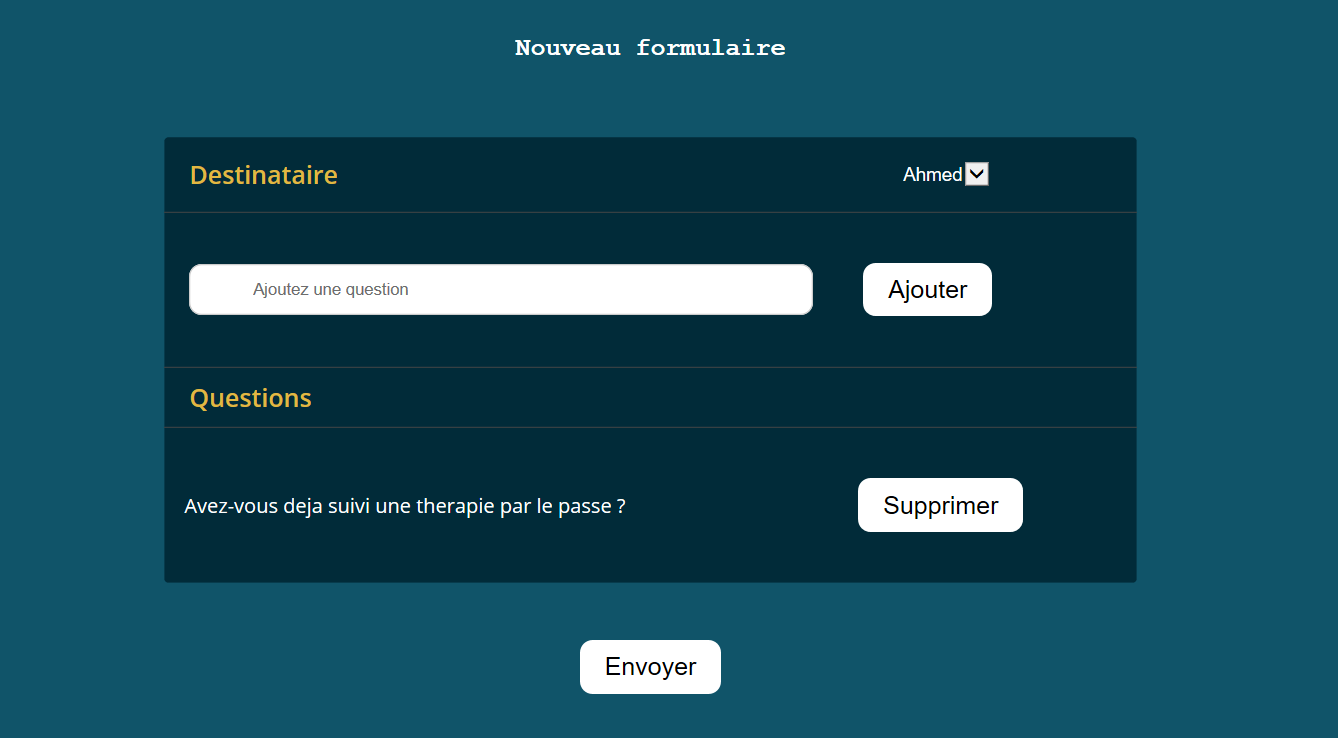
\includegraphics[scale=0.4]{C:/Workplace/Java/project/26.PNG}
\captionof{figure}{Nouveau Formulaire}
\end{center}


Au cas de l'envoie 


\begin{center}
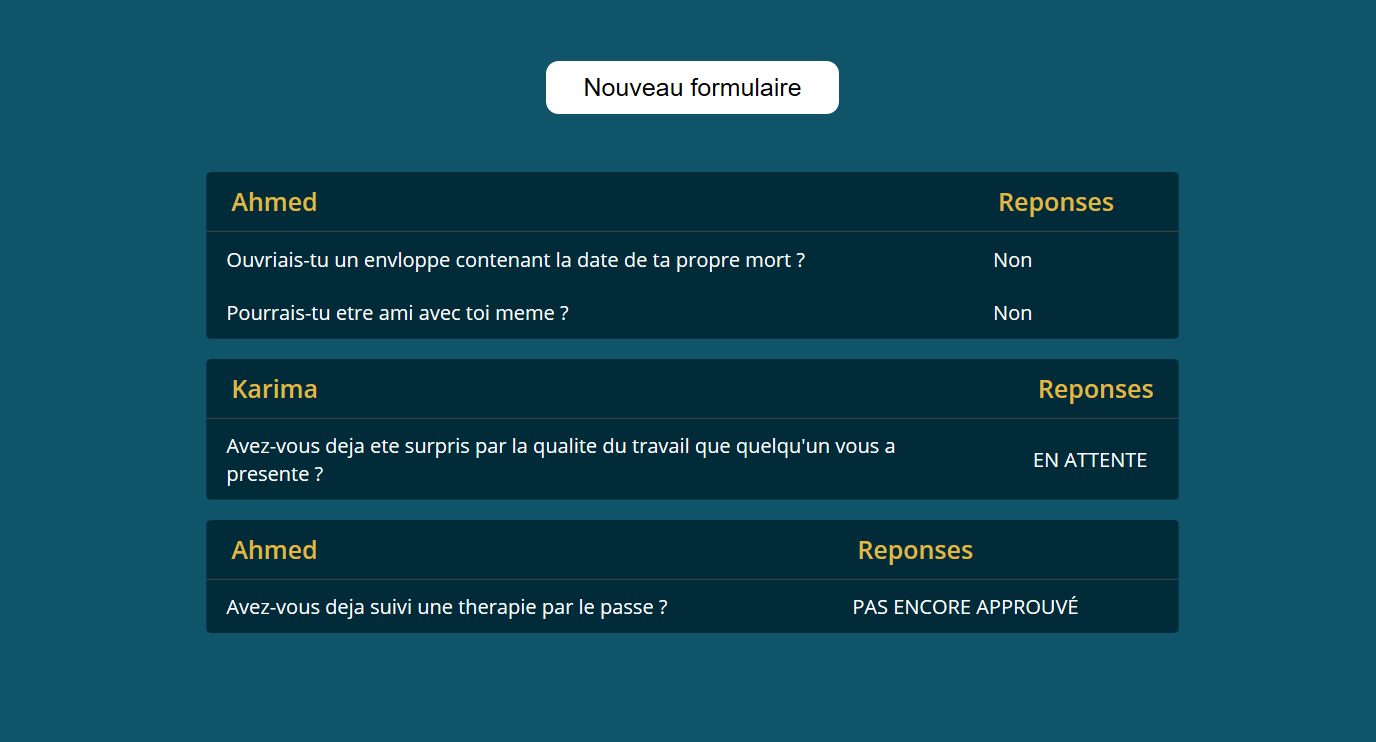
\includegraphics[scale=0.4]{C:/Workplace/Java/project/27.PNG}
\captionof{figure}{Interface psychologue}
\end{center}

Le formulaire serait aussi affiché chez le RH.



\begin{center}
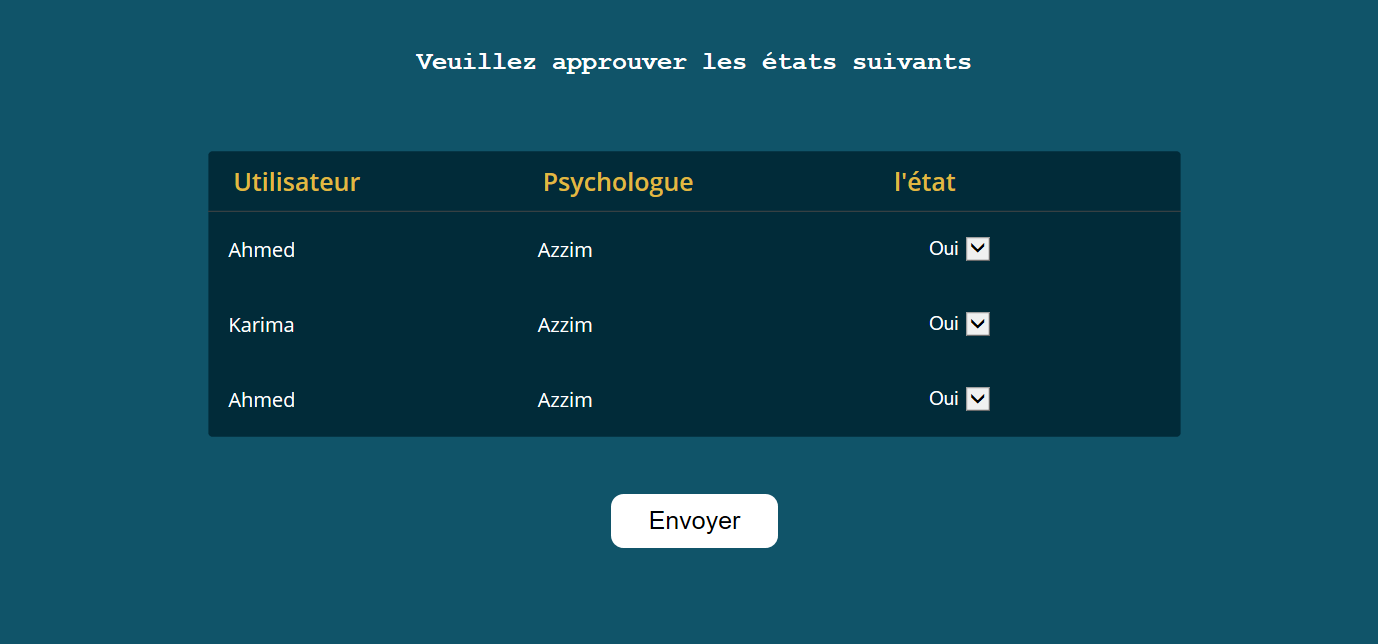
\includegraphics[scale=0.4]{C:/Workplace/Java/project/28.PNG}
\captionof{figure}{Interface RH}
\end{center}


Au cas de l'approuvement la question serait affichée à l'utilisateur



\begin{center}
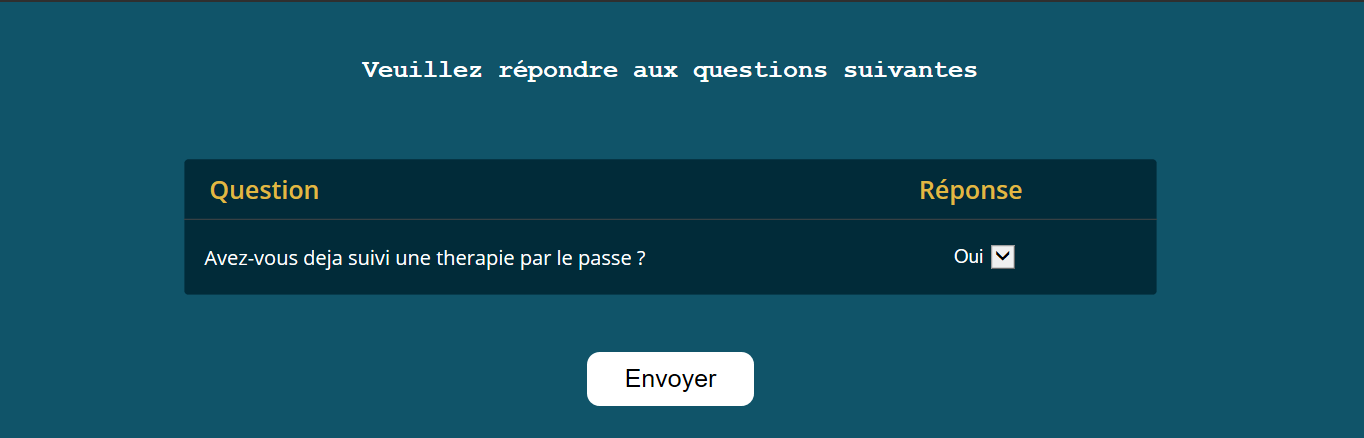
\includegraphics[scale=0.4]{C:/Workplace/Java/project/29.PNG}
\captionof{figure}{Interface Utilisateur}
\end{center}




\subsection{Ajustement des recules}

Un problème qui viens d'apparaitre pour le psychologue est le retour vers la page des formulaires après avoir ajouter un nouveau.\\


Une solution consiste à transférer le code du psychologue vers la méthode \textit{doget()}. Cela va permettre au bouton du retour de prendre comme action la méthode "get" au lieu de "post".\\

La serlvet login serait donc comme suit 



\begin{scriptsize}
\lstset{language=java}
\begin{lstlisting}
@WebServlet("/login")
public class LoginServlet extends HttpServlet {

	protected void doGet(HttpServletRequest request, HttpServletResponse response)
			throws ServletException, IOException {
		List<Formulaire> formulaires = new ArrayList<Formulaire>();
		List<Question> userquestion = new ArrayList<Question>();
		DB connexion_db = new DB();
		Session session = new Session();

		session.affecteNom(request.getParameter("nom"));

		connexion_db.liste_formulaire_psychologue(session.returnNom(), formulaires);
		connexion_db.question_utilisateur_psychologue(session.returnNom(), userquestion);
		request.setAttribute("psy", session.returnNom());
		request.setAttribute("userquestion", userquestion);
		request.setAttribute("formulaires", formulaires);
		RequestDispatcher rst = request.getRequestDispatcher("Psychologue.jsp");
		rst.forward(request, response);
	}

	protected void doPost(HttpServletRequest request, HttpServletResponse response)
			throws ServletException, IOException {
		String nom = request.getParameter("nom");
		String passe = request.getParameter("mot de passe");

		Session session = new Session();
		session.affecteNom(nom);
		session.affectePasse(passe);
		DB connexion_db = new DB();
		if (connexion_db.valider_donees(session)) {
			if (session.returnType().equals("Psychologue")) {
				doGet(request, response);
		.
		.
		.
		.

\end{lstlisting}
\end{scriptsize}




Finalement le bouton retour fait appel à la méthode \textit{get} et indique le nom du psychologue en tant que hidden input.

\begin{scriptsize}
\lstset{language=XML}
\begin{lstlisting}
<form class = login action="login" method="get">
<button type="submit" value="Login" class = "logout">Retour</button>
<input type="hidden" name="nom" value="${psy}" />
</form>
\end{lstlisting}
\end{scriptsize}




























\end{document}